\documentclass[twocolumn, ]{article}
\usepackage{amsmath}
\usepackage{graphicx}
\usepackage{geometry}
 \geometry{
 a4paper,
 total={170mm,257mm},
 left=10mm,
 top=10mm,
 }
 \usepackage{setspace}
\setstretch{0.3}

\begin{document}

\section*{\small Cheat Sheet for EE463}

\subsection*{\small Performance Parameters}
\begin{equation*}
Form Factor=\frac{V_{rms}}{V_{avg}}
\end{equation*}
\begin{equation*}
Crest Factor=\frac{V_{peak}}{V_{rms}}
\end{equation*}
\begin{equation*}
Distortion Factor=\frac{I_{1rms}}{I_{rms}}
\end{equation*}
\textit{$\phi$ : phase difference between fundamentals of current and voltage}
\begin{equation*}
Displacement Power Factor=\cos(\phi)
\end{equation*}
\begin{equation*}
True Power Factor=\frac{P}{S}=DPF \frac{I_{1,RMS}}{I_{RMS}}
\end{equation*}
\begin{equation*}
THD=\sqrt{(\frac{I_{rms}}{I_{1rms}})^2-1}
\end{equation*}



\subsection*{\small Single Phase Diode Rectifier}

\begin{equation*}
	V_{av}=\dfrac{2 \sqrt{2}V_{s}} { \pi}
\end{equation*}

\textit {u: commutation period}
\begin{equation*}
 	\cos(u)=1-\dfrac{2\omega L_{s} I_{d}}{\sqrt[]{2}V_{s}}
\end{equation*}

\begin{equation*}
 	\\ Id\_{av}= \dfrac{\int_b^f i(\theta) d \theta}{\pi}  \\
\end{equation*}

\begin{equation*}
 	\\ Id\_{(short-circuit)} = \dfrac{Vs}{\omega Ls}\\ 
\end{equation*}

\begin{figure}[!ht]
	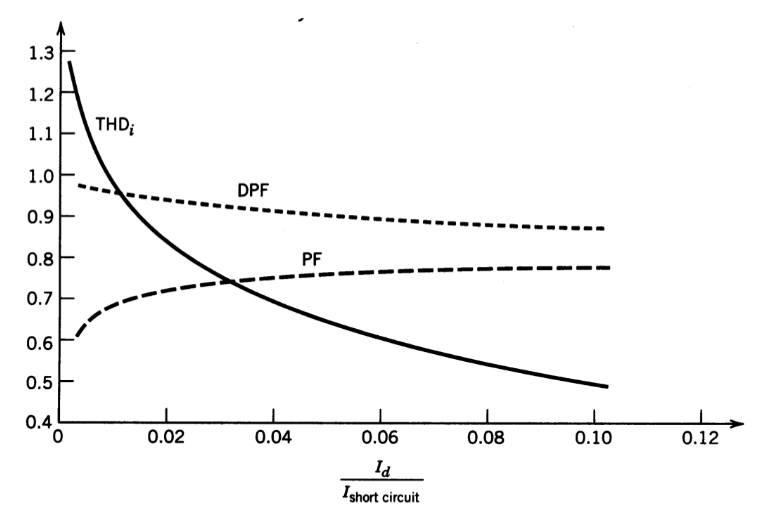
\includegraphics[scale=0.45]{avcur}
	\caption{Characteristics of source current wrt w*Ls (battery on load side)}
\end{figure}

\subsection*{\small Three Phase  Rectifier}

\begin{itemize}



\item \textbf{Half Wave} 
\begin{equation*}
	V_{av}=\dfrac{3 \sqrt{6}V_{s}} {2 \pi}
\end{equation*}
Crossing points (integration) on the waves are from $\pi /6$ to $5 \pi /6$

 

\item \textbf{Full Wave} 

\textit{Full Bridge Rectifier Average Output $V_{s}$:rms value of source voltage}
\begin{equation*}
 	V_{av}=\frac{3 \sqrt{6} V_{s}}{\pi }-\frac{3wL_{s}I_{d}}{\pi }
\end{equation*}

{\small Thyristor}
\textit{$\alpha$ : firing angle}

\begin{equation*}
	V_{av}(\alpha)=\frac{3 \sqrt{6} V_{d}}{\pi }-\frac{ 3 \sqrt{6} V_{d}}{\pi }\cdot (1-\cos(\alpha))
\end{equation*}

\begin{equation*}
	V_d = 0.9 V_s cos(\alpha) - \dfrac{2\omega L_s I_d}{\pi} \\
\end{equation*}

\textit{At the output $I_{d}$}
\begin{equation*}
	\cos(\alpha + u)=\cos(\alpha)-\dfrac{2\omega L_{s} I_{d}}{\sqrt[]{2}V_{s}}
\end{equation*}

\end{itemize}

\subsection*{ \small Trigonometric }

\begin{align*}
          \sin A \cos B &= \frac{1}{2}\left[ \sin(A-B)+\sin(A+B) \right] \\
          \sin A \sin B &= \frac{1}{2}\left[ \sin(A-B)-\cos(A+B) \right] \\
          \cos A \cos B &= \frac{1}{2}\left[ \cos(A-B)+\cos(A+B) \right] \\         
	  \[cos A + cos B = 2\cos(\frac{A+B}{2})\cos(\frac{A-B}{2})\]
	  \[cos A - cos B = (-2)\sin(\frac{A+B}{2})\sin(\frac{A-B}{2})\]
	  
\end{align*}


\end{document}
